\chapter{Learning speech acts}
\label{chap:eng-sp}
As we have discussed in the last two chapters, pragmatics is crucial for children to learn clause type categories, and even noisy pragmatics can benefit the learner. But then, there still remains the question of how children learn speech act categories? Given that the way we generally identify a speech act is via its clause type, there is a potentially vicious circle here: you need to know the clause type to identify the speech act, but you need to know the speech act to identify the clause type. How do learners avoid this circularity? While clause type information might be important for speech act recognition, it is possible that the learner has access to other non-clause type cues that might be helpful to recognize some, possibly noisy, pragmatic information. This chapter therefore explores whether such cues are present in children's input, and how informative these cues are to speech act information. If children use these cues to infer speech act, would the noise level in their inference be below 80\% (and 40\% for Mandarin learners), so that they can use this information to learn clause type clustering? 

Previous studies have investigated the possible behavioral patterns associated with speech acts. For example, \textcite{domaneschi2017facial} find that the upper half of the face is related to the performance of speech acts. But due to the nature of the data recorded in the Providence corpus (\citealt{ProvidenceCorpus}), we are limited in the types of cues we can explore. In this chapter, I will focus on three types of cues: prosody, speech gaps, and attentional behavior. 


As we have discussed in Chapter~\ref{chap:background}, one way of understanding speech acts is to look at their effects on the discourse. Specifically, the effect of questions and requests are different from assertions; the first two require the engagement of an addressee, either to provide responses or perform action, but assertions do not have such requirements. This discourse effect makes questions perfect turn-transition points (\cite{duncan1972turn} among many others), signaling that the current speaker is done with the turn and the next speaker needs to get ready. As speakers tend to use signals like eye gaze to appoint the next turn, these signals might be useful for identifying which utterances are questions. 

Another similar conversational signal might be the turn-taking time. A property related to a turn-transition point is that interlocutors use these points as cues for when to take over the turn. In a natural face-to-face conversation, the gap between a question and its answer might be smaller than other pairs of utterances in a conversation (\citealt{tice2011turn} a.o.). But the questioner might also pause and wait if nobody steps in immediately (\cite{sacks1978pause}). Therefore, tracking the gap after utterances might tell us whether the utterance is a question.

As for prosodic cues, we have discussed in Chapter~\ref{chap:background} that rising contour tends to be associated with questions cross-linguistically (\cite{gussenhovenchen2000}). We are then interested in how parents use prosody in speech to children.

This chapter is organized as follows: Section~\ref{sec:engsp:background} reviews previous evidence for children's perception of these cues. I then report results from a corpus study with Providence Corpus in Section~\ref{sec:engsp:corpus}, where I looked at the prosody of parents' utterances (Section~\ref{sec:engsp:results:prosody}), the speech gap between parents' utterances (Section~\ref{sec:engsp:results:pause}), and parents' attentional behavior (\ref{sec:engsp:results:gaze}).
Section~\ref{sec:engsp:discussion} concludes the chapter.


\section{Background}
\label{sec:engsp:background}
\subsection{Prosody}
\label{sec:engsp:bg:prosody}
As we have seen in Chapter~\ref{chap:background}, rising intonation tends to associate with interrogatives (particularly polar interrogatives) and questions cross-linguistically. Results from previous experimental and corpus studies suggest that children might be sensitive to the distinction between a final rise (specifically polar interrogative rise) and a final fall. 

From as early as 6 months old, infants are able to identify utterance boundaries, and are sensitive to the edge prosody (\cite{johnson2014edge}). They also can use distinctions in prosodic contours (e.g. final rise vs. fall) to distinguish clause types (polar interrogative vs. declaratives). For example, \textcite{frota2014}) show that as young as 6 months old, European Portuguese-acquiring infants are sensitive to the prosodic distinction between polar interrogatives and declaratives, where prosody is the only cue that distinguishes these two clause types in the language. \textcite{geffenmintz2011} find that when given a combination of word order and prosodic cues, English-acquiring 7-month-olds can distinguish polar interrogatives from declarative assertions. \textcite{soderstrom2005clause} test English-speaking infants between 4.5 months and 2 years old (average 14 months old), and find that they are sensitive to the distinction between declaratives with a falling a rising contour. Before 18 months old, infants acquiring non-lexical tone languages such as English are shown to be sensitive to some tonal distinctions in lexical tone languages such as Mandarin. They are particularly sensitive to the distinction between the rising tone that is similar to English polar-interrogative rise, and the falling tone similar to English declarative fall (\cite{shi2017tone, Hay2019}).%, although it is unclear whether we can draw any conclusions about their sensitivity to English polar interrogative rise.

While infants might be sensitive to the distinction between rise and fall, it is unclear, at least for English-acquiring infants, whether they can use prosodic cues alone to detect questions. When given only prosodic cues without any morpho-syntactic information, \textcite{keitel2013turn} and \textcite{casillas2017turn} both find that children younger than 2 years old cannot use intonation alone to infer transition after a turn, but they can infer such transitions with morpho-syntactic cues associated with interrogatives. 

On the production side, studies have found that children are able to use different prosodic contours for different functions from when they start speaking. \textcite{menyuk1969prosody} analyze the prosodic contours of one child's utterances, and annotates their perceived speech acts between 18  and 20 months, and find that even though the utterances are mostly one word or two words, there's a correlation between the intended speech act and prosody. For example, an intended request with a one-word utterance ``door!'' is typically associated with a sharp rise and then fall; the same utterance as a question tends to end with a rising intonation. Since the speech act labels in the study are annotations by adults inferred from one-word utterances, it is unclear whether these are actually the speech acts that the child perform, and the conclusion seems to be that adults systematically associate certain prosodic contours to \aqrs{}, even with one-word utterance. Nonetheless, it seems that at the child is using different prosodic contours at this age, and it is possible that these contours are systematically associated with different speech acts. 

Furthermore, for their own production, children seem to associate the rising contour with response elicitation. \textcite{flax1991prosody} conduct a longitudinal study observing three children interacting with their mothers before they can speak (when they have a vocabulary of 10 words, and again when their vocabulary consists of 50 words), and code whether the child's utterance (or vocalization, at the pre-verbal stage) is produced with a final rise. They find when children request a response from their addressee, they tend to produce the utterance with a final rise. 

Previous studies have also shown that there are prosodic cues that distinguish clause types and speech acts, in particular to distinguish polar interrogatives and declaratives, in child-directed speech. \textcite{geffenmintz2017final} show that polar interrogatives and declaratives differ in the pitch of the last two syllables, with polar interrogatives generally have a rising contour; they also find that there is no distinction between \twh-interrogatives and declaratives in the last two syllables. \textcite{chianggeffenmintz2018initial} examine sentence-initial prosodic cues, and find that polar interrogatives and declaratives both have a higher starting pitch than declaratives, and that echo \twh-questions tend to have a higher pitch than other types of questions. %These studies only looked at the duration, F0, and intensity of the last two and the first syllables; there might be 

In sum, prosodic cues are in principle helpful for distinguishing different speech acts, and there is evidence suggesting that children can perceive these cues. In particular, there might be cues at sentence-final and sentence-initial position that are both useful and available to children. We will examine the role of prosody more closely in Section~\ref{sec:engsp:corpus}, where we also discuss possible cues that go beyond the last two and the first syllables.

\subsection{Pauses in conversation}
\label{sec:engsp:bg:pause}
As mentioned earlier, questions are turn-transition points (\cite{duncan1972turn} among others), and this means that speakers anticipate a change of turn after questions. In adult-to-adult conversations, this property translates to shorter speech gaps after questions in one-on-one in-person conversations (\cite{stivers2010,enfield2010,hilbrink2013turn} among many others). Speakers might also wait after questions for responses (\cite{sacks1978pause}), but for adults, longer inter-turn silence leads to feelings of unease and tend to be avoided (\cite{roberts2006pause} among others). But when interacting with pre-linguistic infants, this silence might be helpful rather than awkward: if children can track the length of pause after an utterance, they might be able to infer that longer pauses are associated with questions and request. Are children sensitive to the turn-taking properties of conversations? 
%As infants could use prosodic cues to detect clause boundaries (\cite{hirsh1987clause, seidl2007prosody}), they might be able to track the length of pause after an utterance. 

As early as 3 months old, infants show sensitivity to the structure of conversation. The overlap between infant vocalization and parents' speech decreases overtime, and the average gap between parent utterance and infant vocalization decreases, suggesting that they respect the turn-taking rules (\cite{hilbrink2013turn3mo}). When they start producing one-word utterances, slow down at trying to change turn, but quickly pick up the speed again as their linguistic ability develops (\cite{hilbrink2013turn}).

Studies also show that same as adults, children interpret pauses as meaningful. \textcite{craiggallagher1983pause} 
investigate whether or not 22-36-month-olds abandon their request (e.g. wanting a cookie) after the parent's initial responses (classified as neutral, e.g. \tit{you want what?},  negative, \tit{No.} or pause). They found that the older children (3-year-olds) abandon requests after adult pauses for more than 1s, suggesting that children treat long pauses as a meaningful response. This is suggestive, but based on this research alone it remains unclear whether children associate inter-turn silence with the interlocutor trying to elicit a response. 

%Bloom et al: four children, 21 to 36 months of age. Adjacent speech is more than anything from the beginning, Contingent speech increase over time (adjacent (immediately preceded by an adult utterance), or as nonadjacent (not immediately preceded by an adult utterance). Adjacent utterances were either contingent (shared the same topic and added new information relative to the topic of the prior utterance), imitative (shared the same topic but did not add new information), or noncontingent (did not share the same topic). Linguistically contingent speech (speech that expanded the verb relation of the prior adult utterance with added or replaced constituents within a clause)  occurred more often after questions than nonquestions. 

On the other side the problem, the length of pauses results from the dynamics of conversation; if parents are interacting with a pre-linguistic infant, would they follow the same rules? In other words, if we assume that children can keep track of the length of pauses, are there any patterns found in the silences? Previous studies show that parents seem to treat even pre-linguistic infants as competent conversationalists, and any vocalizations (e.g. crying, babbling) or even body movements, are treated as a conversational turn (\cite{beebe1988,jaffe2001turn}). The length of pauses also correlates with the vocabulary of children (\cite{marklund2015pause}). Different from adult-to-adult interactions, parents of 14-month-olds tend to follow questions with another question (\cite{reimchen2017}).  

While these studies show that parents respect turn-taking rules when interacting with pre-verbal infants, little is known about whether parents' speech gaps are informative of the speech act performed. To address this problem, Section~\ref{sec:engsp:results:pause} examines the correlation between the speech act of an utterance and the length of pauses after an utterance, to see if the gap between utterances is informative of an utterance's speech acts. 

\subsection{Attentional behavior}
\label{sec:engsp:bg:gaze}

Another consequence of the response-expectation property of questions is that by the end of a question, the speaker tends to appoint the next speaker. A common device for turn allocation is eye gaze (\citealt{argyle1972gaze, kendon1967gaze,duncan1979gaze, rossano2009gaze, csibra2010}). In dyadic interactions, we tend to look at our interlocutor when we need their response. Thus, it is possible that by tracking where the parent attends to, specifically whether the parent is directly looking at the learner, the learner might be able to infer whether a question is being asked. 

We have seen in Chapter~\ref{sec:bg:acq:pre} that infants are sensitive to the direction of eye gaze since birth. 3-day-old newborns prefer to look at the face that appears to make eye contact with them, suggesting that they are sensitive to the position of the pupils/irises within the eye (\cite{farroni2004gaze}).


While these studies show that infants can perceive parents' direction of eye gaze, and that adults use eye gaze for turn allocation, so far little is known about whether parents' gaze pattern correlates with turn allocation, and furthermore, with the speech act of an utterance. If questions signals a transition of turn, parents' gaze should fall on the addressee--the child--more after questions. I address this question in Section~\ref{sec:engsp:results:pause} by examining parents gaze pattern during parent-child interactions, to see if this cue is informative of an utterance's speech acts.

\subsection{Interim Summary}
\label{sec:engsp:bg:summary}

When interacting with other people, we use many cues, besides the clause type information, to infer what kind of speech act is being performed. In particular, since questions usually signal the transition of a conversational turn, the questioner usually shifts gaze to the next designated speaker. Adults can also infer from a question being performed that the questioner wants someone to pick up the turn, and thus the lengths of speech gap after questions are normally longer than lengths of pause after other speech acts. However, if we look at dyadic interactions between a parent and a child, especially a child as young as 18 months old, these cues might not show up, or show up in a different way. We should ask, for example, whether parents in child-directed interaction also use direct eye gaze to indicate the next speaker, i.e. the child? Also, since 18-month-olds are not mature conversationalists, the speech gap after utterances might be longer across the board, so are there any differences in pauses that correlate with the speech act being performed? Another potential cue is prosody. In English, yes/no questions are usually associated with a special final rise contour (L* H-H\%), which can be produced with either polar interrogatives and declaratives syntax. Would final rises be a cue that distinguishes between the three speech acts?

To address these questions, we built a multi-modal dataset with dyadic parent-child interactions for infants before 18 months old, to see if there is any non-clause type cues that may help infants distinguish speech acts.

\section{Corpus study}
\label{sec:engsp:corpus}

This section details the corpus study we conducted to investigate whether speech gap, direct gaze, and prosody in dyadic parent-child interactions correlate with parents' use of different speech acts. 


\subsection{Methods}
\label{sec:engsp:corpus:method}
This study also used data from the Providence Corpus (\citealt{ProvidenceCorpus}) from CHILDES system (\citealt{CHILDES}). The audio and video of the sessions sampled in Chapter~\ref{chap:eng-cl} were extracted for annotation. 

For the audio data, I adapted a Kaldi forced alignment system (\cite{kaldi}) to obtain a time-aligned dataset containing the beginning and ending timestamp of each utterance in a session. I also manually aligned 20\% of this dataset to compare for accuracy. The mean difference between the manually aligned dataset and the forced-aligned dataset is 0.1s at the beginning of the utterance (0.001s to 20s), and 0.08s at the end of the utterance. We then extracted the pitch information of each utterance using Praat (\cite{praat}). 

For annotating gaze, we used the video data available in the Providence corpus. Trained annotators viewed the muted videos using ELAN (\cite{elan}). Each video was annotated first with whether the parent and the child are visible on screen and the parent's focus of attention can be identified. If the parent is only half on screen, but we can still identify the focus of attention of the parent, this proportion was counted as on-screen. If the parent is on screen but the focus cannot be identified due to bad lighting, this proportion of the video was counted as off-screen.

Then, for the parts of the video that both the parent and the child are both on screen, the focus of parents' attention was annotated. Specifically, whether the parent is paying attention to the child, to an object, or unidentifiable. The parent was annotated as paying attention to the child when they attended to the child through (1) direct eye gaze (when the eyes could be seen), (2) head or body orientation toward the child (when the eyes could not be seen), (3) physical interaction with the child.  

I then used a script to calculate the proportion of looks to the child during the utterance, and at 1s, 2s, 3s before and after the utterance.%, by dividing the total length of the on-screen time by the length that the parent attends to the child.  

\subsection{Predictions}
\label{sec:engsp:predictions}
If prosody, speech gaps and gaze are indeed useful cues to obtain speech act information, we would expect the following predictions to bear out.

For prosodic patterns, we should see that final rising contour is more frequently associated with questions, especially polar interrogatives, than with assertions.
For speech gaps, we should see that parents pause longer after questions and requests than after assertions, to wait for responses.
And for eye gaze, we should see that parents direct attention to the child more often after questions and requests than after assertions. 


\subsection{Results}
\label{sec:engsp:results}

\subsubsection{Prosody}
\label{sec:engsp:results:prosody}
The pitch information from 5430 utterances were extracted by using Praat (\citealt{praat}). I further applied a low-pass filter at 500 Hz that removes most of the phonetic information used to distinguish between phonemes. From this pitch data, to approximate the process of finding the last pitch accent in the utterance, I applied a peak/valley identification algorithm. The last peak or valley was then considered the last pitch accent. If it's a peak like (\ref{fig:rise-example}), then the utterance was labelled as having a final rising contour. The script for coding pitch information can be found at \mycode{}. We manually annotated 40 utterances to check for accuracy; 27 of these were correctly labeled by the algorithm.  


\begin{figure}[H]
    \centering
    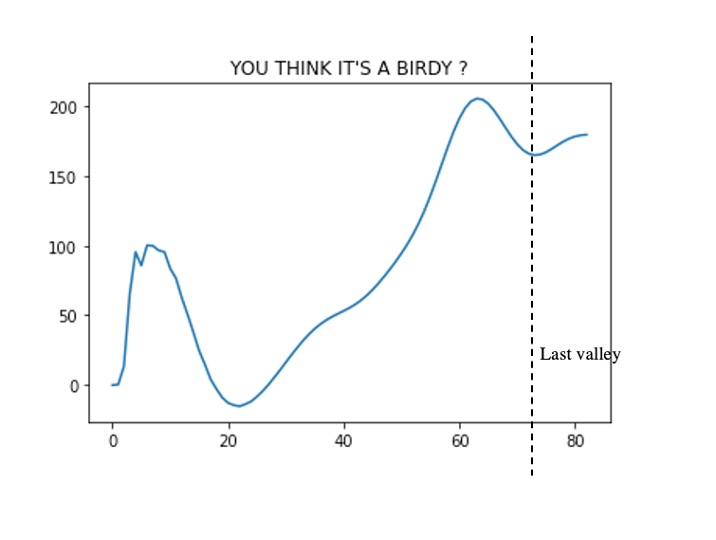
\includegraphics[width=0.7\textwidth]{figures/pitch-rise.jpg}
    \caption{``You think it's a birdy?''}
    \label{fig:rise-example}
\end{figure}

Figure~\ref{fig:rise-sp} and \ref{fig:rise-cl} show the proportion of final rise, as identified by the algorithm. As we can see, there is no difference in the proportion of rises among speech acts. 

\begin{figure}[H]
    \centering
    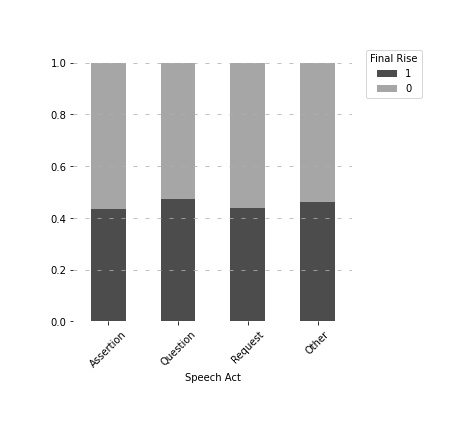
\includegraphics[width=0.7\textwidth]{figures/rise-sp.jpg}
    \caption{Proportion of utterances with final rise across different speech acts}
    \label{fig:rise-sp}
\end{figure}


\begin{figure}[H]
    \centering
    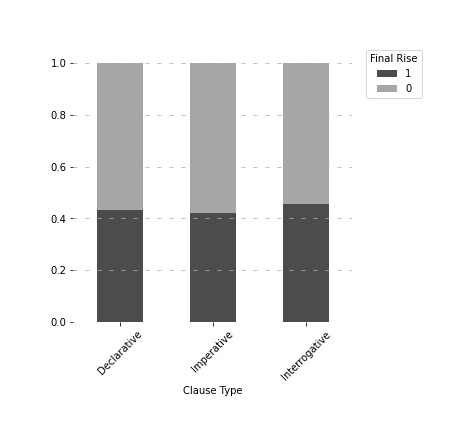
\includegraphics[width=0.7\textwidth]{figures/rise-cl.jpg}
    \caption{Proportion of utterances with final rise across different clause types}
    \label{fig:rise-cl}
\end{figure}

But if we look into sub-categories of interrogatives, we can see that the proportion of final rise is much higher with polar interrogatives than with declaratives. 
\begin{figure}[H]
    \centering
    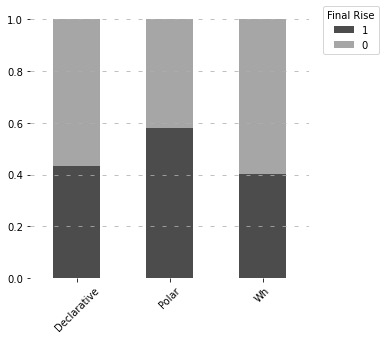
\includegraphics[width=0.7\textwidth]{figures/pitch-polardecwh.jpg}
    \caption{Proportion of declaratives, \twh{} and polar interrogatives with final rise}
    \label{fig:rise-int}
\end{figure}

These results seem to suggest that the presence of final rise might not be informative of the speech act of the sentence, unless morpho-syntactic features like subject-auxiliary inversion is also present. However, this could be a result of the algorithm I applied here, and do not reflect the pattern of the data. I plan to hand annotate more cases in the future to have more reliable data.

\subsubsection{Pauses}
\label{sec:engsp:results:pause}

For this cue, we measured the length of silence between parents’ consecutive utterances like (\ref{code-prag:pause}). To do so, we first followed the methodology of \textcite{bloom1976discourse} and annotated for each utterance whether it is a contingent utterance of the previous one, i.e.\ whether it shares the same topic and adds new information relative to the topic of the prior utterance. We will refer to such pairs of utterances, with one contingent on the previous utterance like in (\ref{code-prag:pause}), as consecutive turn sequences. Within the sequences, I measured the length of pauses between utterances. 


\bex{code-prag:pause}
%\bxl{}
\tbf{Consecutive turn sequence}
\bxl
You can’t take your rake on the swing.\\
 \tsc{pause: 0.014s} \\ 
 You wanna take your big bird rake on the swing? 			\hfill \tsc{Assertion -Question}
\ex You don't wanna swing?\\
 \tsc{pause: pause: 0.23s} \\	
 You don’t have to.	\hfill \tsc{Question-Assertion}
\ex Here you use this one. \\
 \tsc{pause:  0.033s} \\ This one works better.	\hfill \tsc{Assertion-Assertion}
\exl
\eex

In total, 4066 utterances were found to have a contingent follow-up that allows us to measure the inter-turn silence. Figure~\ref{fig:engsp:pause} shows the length of pause after each speech act category.

\begin{figure}[H]
\begin{center}
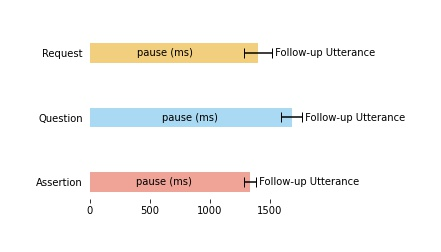
\includegraphics[width = 0.8\textwidth]{figures/pause.jpg}
	\caption{Duration of pause (ms) after each type of speech act}\label{fig:engsp:pause}
\end{center}
\end{figure}

These results show that parents are equally likely to ask another question as they are to answer their own questions, but parents tend to pause longer after questions (mean $= 1728ms$) than assertions (mean $= 1321ms; t(2925) = -2.23, p = 0.02$), suggesting that parents pause after asking a question but proceed with the conversation after an assertion. %There is no difference between questions and requests mean $= 1345ms; t(1418) = 0.83, p = 0.4$), suggesting

\begin{comment}
\begin{figure}[H]
\begin{center}
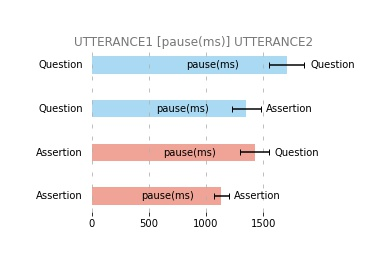
\includegraphics[width = 0.8\textwidth]{figures/pause-QA.jpg}
	\caption{Duration of pause (ms) between Question-Question/Assertion and Assertion-Question/Assertion pairs }\label{fig:engsp:pause-QA}
\end{center}
\end{figure}
\end{comment}


\subsubsection{Parents' attentional behavior}
\label{sec:engsp:results:gaze}

In total, 857 utterances were found to have attentional data suitable for annotation. Figure~\ref{fig:attention} shows the proportion of looks to the child before, during, and after an utterance.


\begin{figure}[H]

\begin{center}
	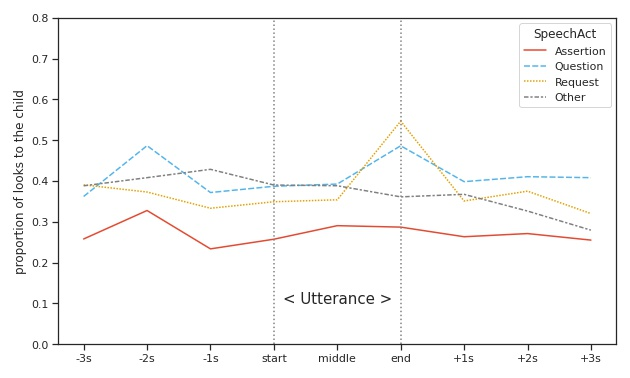
\includegraphics[width =1\textwidth]{figures/gaze-pattern-adult.jpg}
	\caption{Proportion of parents' looks to the child before, during, and after an utterance} \label{fig:attention}
\end{center}
\end{figure}


From Fig.~\ref{fig:attention}, we can see that when the utterance is a question, the proportion of looks to the child is higher (average $0.41$) than when it is an assertion (average $0.27; t(16) = 2.53, p <0.05$), but roughly equivalent to when the utterance is a request ($0.37; t(16)= 1.27, p=0.21$); in the post-utterance region, the proportion of looks to the child is higher when the utterance is a question ($0.53$) than when it is an assertion ($0.25; t(4) = 7.95, p<0.05$) but not when it's a request ($0.39; t(4) = 4.2, p=0.2$). These results suggest that parents look at the child longer after questions and requests. %%%%


\subsubsection{Informativeness of the cues}
\label{sec:engsp:results:stats}
A multinomial logistic regression model was built with the three cues as independent variables, and the speech act categories (assertions, questions, requests, and other) as the dependent variable. The data for the model was an intersection of the prosody, pause, and attentional data, as not all utterances have follow-up utterances for us to measure the inter-turn silence, and some utterances were uttered off screen with no attentional data. In total, 806 utterances were included in the analysis.  We then split the data into a training set (90\% of the data) and testing set (10\%), and trained a logistic regression classifier with the training data. For details of the model, see Appendix~\ref{appx}. This classifier can predict 57\% of the speech act labels, suggesting that the three cues could to some extend help children identify speech act information. 

\section{Conclusion}
\label{sec:engsp:discussion}
In this chapter, we addressed the question of how children learn to identify speech acts, specifically, we looked at whether certain non-clause type cues, such as prosody, speech pauses, and attention, could help the learner identify speech acts. With a corpus study, I showed that it is possible to get some knowledge related to the identifcation of speech act type from these three cues. Specifically, polar questions tend to be associated with a rising intonation; parents pause longer after questions and requests; and they look at the child longer when asking questions. 



%Note that at this point I do not claim that 18-month-olds use there cues for speech act identification, but merely probing into whether this information is present in the corpus. 
%Information is present, but do speakers in fact extract speech act information from these cues?
%Human Simulation Paradigm 
%( \cite{trueswell2016hsp})
%Are these cues enough? Modeling. Problem right now: not enough data